% ╔══════════════════════════════════════════════════════════════════╗
% ║  Мобильная версия — iPhone 12 Pro (90×195 мм)                   ║
% ║  xelatex self_evolving_flow_mobile.tex                          ║
% ╚══════════════════════════════════════════════════════════════════╝

\documentclass[10pt, oneside]{article}

% ─── Шрифты и язык ───────────────────────────────────────────────
\usepackage{fontspec}
\usepackage{polyglossia}
\setdefaultlanguage{russian}
\setotherlanguage{english}
\setmainfont[
  Ligatures=TeX,
  BoldFont={Liberation Serif Bold},
  ItalicFont={Liberation Serif Italic}
]{Liberation Serif}
\setsansfont[Ligatures=TeX]{Liberation Sans}
\setmonofont[Scale=0.78]{DejaVu Sans Mono}

% ─── Страница — точно под iPhone 12 Pro ─────────────────────────
% Экран: 2532×1170 px @ 460ppi → 139.6×64.0 мм
% PDF-страница с полями: 90×195 мм
\usepackage[
  paperwidth=90mm,
  paperheight=195mm,
  top=7mm,
  bottom=7mm,
  left=7mm,
  right=7mm,
  headheight=0pt,
  headsep=0pt,
  footskip=5mm
]{geometry}

% ─── Базовые пакеты ──────────────────────────────────────────────
\usepackage{parskip}
\usepackage{setspace}
\usepackage{booktabs}
\usepackage{array}
\usepackage{tabularx}
\usepackage{enumitem}
\usepackage{graphicx}
\usepackage{float}
\usepackage{caption}
\usepackage{amsmath}
\usepackage{amssymb}
\usepackage{ragged2e}
\usepackage{needspace}

% ─── Цвета ───────────────────────────────────────────────────────
\usepackage[dvipsnames, svgnames]{xcolor}
\definecolor{AccentBlue}{RGB}{25, 90, 165}
\definecolor{AccentTeal}{RGB}{0, 115, 115}
\definecolor{AccentOrange}{RGB}{190, 70, 0}
\definecolor{LightGray}{RGB}{246, 247, 251}
\definecolor{MidGray}{RGB}{120, 125, 138}
\definecolor{DarkGray}{RGB}{35, 38, 48}
\definecolor{CodeBg}{RGB}{244, 245, 250}
\definecolor{CodeBorder}{RGB}{195, 200, 220}
\definecolor{GreenOk}{RGB}{28, 135, 58}
\definecolor{LinkColor}{RGB}{15, 80, 165}

% ─── Гиперссылки ─────────────────────────────────────────────────
\usepackage[
  unicode,
  colorlinks=true,
  linkcolor=LinkColor,
  urlcolor=AccentTeal,
  citecolor=AccentOrange,
  pdftitle={Саморазвивающийся поток},
  pdfauthor={Opus Research}
]{hyperref}

% ─── Листинги кода ───────────────────────────────────────────────
\usepackage{listings}
\lstset{
  basicstyle=\fontsize{6}{8}\ttfamily\color{DarkGray},
  backgroundcolor=\color{CodeBg},
  frame=single,
  framerule=0.5pt,
  rulecolor=\color{CodeBorder},
  breaklines=true,
  breakatwhitespace=false,
  showspaces=false,
  showstringspaces=false,
  numbers=left,
  numberstyle=\fontsize{5}{6}\color{MidGray},
  numbersep=5pt,
  xleftmargin=10pt,
  xrightmargin=2pt,
  aboveskip=6pt,
  belowskip=4pt,
  tabsize=2,
  escapeinside={(*@}{@*)},
}

\lstdefinelanguage{CommonLisp}{
  morekeywords={defun,defpackage,defparameter,let,let*,cond,when,unless,
                if,and,or,not,progn,dolist,mapcar,mapcan,reduce,sort,
                case,format,in-package,use,export,import,load,
                handler-case,error,return-from,values,multiple-value-bind,
                setf,push,car,cdr,cons,list,remove-if,remove-if-not,
                find,subseq,length,first,loop,with-open-file},
  morestring=[b]",
  morecomment=[l]{;;},
  sensitive=false,
  keywordstyle=\color{AccentBlue}\bfseries,
  commentstyle=\color{MidGray}\itshape,
  stringstyle=\color{AccentOrange},
}

\lstdefinelanguage{JSON}{
  morestring=[b]",
  stringstyle=\color{AccentOrange},
}

% ─── Колонтитулы — только номер страницы внизу ───────────────────
\usepackage{fancyhdr}
\pagestyle{fancy}
\fancyhf{}
\fancyfoot[C]{\fontsize{7}{8}\selectfont\color{MidGray}\thepage}
\renewcommand{\headrulewidth}{0pt}
\renewcommand{\footrulewidth}{0pt}

% ─── Заголовки разделов ──────────────────────────────────────────
\usepackage{titlesec}

\titleformat{\section}
  {\fontsize{10}{13}\bfseries\sffamily\color{AccentBlue}}
  {\thesection.}{0.5em}{}
  [\vspace{1pt}{\color{AccentBlue}\rule{\linewidth}{0.5pt}}\vspace{2pt}]

\titleformat{\subsection}
  {\fontsize{9}{11}\bfseries\color{DarkGray}}
  {\thesubsection.}{0.4em}{}

\titleformat{\subsubsection}
  {\fontsize{8.5}{10}\bfseries\color{AccentTeal}}
  {\thesubsubsection.}{0.4em}{}

\titlespacing*{\section}{0pt}{10pt}{4pt}
\titlespacing*{\subsection}{0pt}{7pt}{2pt}
\titlespacing*{\subsubsection}{0pt}{5pt}{1pt}

% ─── tcolorbox ───────────────────────────────────────────────────
\usepackage{tcolorbox}
\tcbuselibrary{breakable, skins}

\newtcolorbox{infobox}[1][]{
  colback=LightGray, colframe=AccentBlue,
  colbacktitle=AccentBlue, coltitle=white,
  fonttitle=\fontsize{7}{8}\bfseries\sffamily,
  boxrule=0.5pt, arc=2pt, breakable,
  top=3pt, bottom=3pt, left=4pt, right=4pt,
  #1
}

\newtcolorbox{warningbox}[1][]{
  colback=Ivory, colframe=AccentOrange,
  colbacktitle=AccentOrange, coltitle=white,
  fonttitle=\fontsize{7}{8}\bfseries\sffamily,
  boxrule=0.5pt, arc=2pt, breakable,
  top=3pt, bottom=3pt, left=4pt, right=4pt,
  #1
}

\newtcolorbox{successbox}[1][]{
  colback=Honeydew, colframe=GreenOk,
  colbacktitle=GreenOk, coltitle=white,
  fonttitle=\fontsize{7}{8}\bfseries\sffamily,
  boxrule=0.5pt, arc=2pt, breakable,
  top=3pt, bottom=3pt, left=4pt, right=4pt,
  #1
}

% ─── Прочее ──────────────────────────────────────────────────────
\newcolumntype{L}{>{\raggedright\arraybackslash}X}
\renewcommand{\arraystretch}{1.25}
\setlength{\parskip}{4pt}
\setlength{\parindent}{0pt}
\captionsetup{font=scriptsize, labelfont=bf}

% Уменьшить отступы списков
\setlist{nosep, leftmargin=1.2em, topsep=2pt}

% ═══════════════════════════════════════════════════════════════════
\begin{document}

% ─── Обложка ─────────────────────────────────────────────────────
\thispagestyle{empty}
\vspace*{8mm}

{\color{AccentBlue}\rule{\linewidth}{1.2pt}}
\vspace{3mm}

{\sffamily\fontsize{7}{9}\color{MidGray} ТЕХНИЧЕСКОЕ ИССЛЕДОВАНИЕ}\\[3mm]

{\sffamily\fontsize{12}{15}\bfseries\color{AccentBlue}
  Саморазвивающийся\\поток
}\\[2mm]

{\sffamily\fontsize{8}{10}\color{DarkGray}
  Архитектура обучающейся системы\\
  в \texttt{development\_system}
}

\vspace{4mm}
{\color{AccentBlue}\rule{\linewidth}{0.4pt}}
\vspace{4mm}

{\fontsize{7.5}{10}\itshape\color{DarkGray}
  Четыре взаимосвязанных потока~--- \textbf{память},
  \textbf{обучение}, \textbf{диагностика} и \textbf{автоматор}~---
  накапливают опыт решения задач, распознают паттерны
  и автоматически порождают специализированные потоки
  без перезапуска образа SBCL.
}

\vfill

\begin{tabular}{@{}ll@{}}
  {\fontsize{7}{8}\color{MidGray}Стек:}    & {\fontsize{7}{8} Common Lisp, LLM} \\[1pt]
  {\fontsize{7}{8}\color{MidGray}Версия:}  & {\fontsize{7}{8} 1.0 · 14 марта 2026} \\
\end{tabular}

\vspace{4mm}
{\color{AccentBlue}\rule{\linewidth}{0.4pt}}

{\fontsize{6.5}{8}\color{MidGray}
  Common Lisp · LLM · ICL · Episodic Memory · Few-Shot · GeoDjango
}

\newpage

% ─── Оглавление ──────────────────────────────────────────────────
{\fontsize{8}{10}\tableofcontents}
\newpage

% ═══════════════════════════════════════════════════════════════════
\section{Введение}

\subsection{Постановка задачи}

Инженер ежедневно решает типовые задачи (N+1, PostGIS, геометрии),
тратя время на воспроизведение уже найденных решений.

\textbf{Система проходит три фазы:}
\begin{enumerate}
  \item \textbf{Запоминание} --- пары (проблема $\to$ решение)
  \item \textbf{Имитация} --- распознавание и воспроизведение
  \item \textbf{Автоматизация} --- порождение специализированного потока
\end{enumerate}

\subsection{Контекст}

\begin{tabular}{@{}ll@{}}
  \toprule
  \textbf{Компонент} & \textbf{Роль} \\
  \midrule
  Мастер (SBCL) & Telegram-бот, polling \\
  Поток & \texttt{*.lisp}, функция \texttt{выполнить} \\
  Порождатель & генерирует потоки через LLM \\
  \bottomrule
\end{tabular}

\vspace{3pt}

Ключевое: \textbf{без перезапуска} --- \texttt{compile-file + load}
в живой образ. Метациркулярность: слой генерации = слой исполнения.

% ═══════════════════════════════════════════════════════════════════
\section{Теоретические основы}

\subsection{In-Context Learning}

LLM решает задачи по примерам в промпте без изменения весов:

\begin{lstlisting}[language={},numbers=none,caption={ICL-промпт}]
Пример 1: <проблема> -> <решение>
Пример 2: <проблема> -> <решение>
Новая проблема: <???> -> ?
\end{lstlisting}

\textbf{Свойства ICL:}
\begin{itemize}
  \item Работает без обучения (готовая модель)
  \item Качество растёт до 10--15 примеров
  \item Ближайшие к запросу --- последними
\end{itemize}

\subsection{Fine-tuning vs ICL}

\begin{tabular}{@{}lll@{}}
  \toprule
  & \textbf{Fine-tuning} & \textbf{ICL} \\
  \midrule
  Веса модели & меняются & нет \\
  Стоимость & высокая & токены \\
  Скорость & дни & мгновенно \\
  Forgetting & да & нет \\
  \bottomrule
\end{tabular}

\begin{infobox}[title={Вывод}]
Fine-tuning избыточен. ICL обеспечивает достаточное
качество с мгновенной адаптацией.
\end{infobox}

\subsection{Episodic Memory}

\textbf{MemGPT (2023):} иерархическая память LLM:
\begin{itemize}
  \item Main context --- рабочая (контекстное окно)
  \item Archival memory --- долговременная с поиском
  \item Recall memory --- поиск по словам
\end{itemize}

В нашей системе: \texttt{поток-память} = archival memory.

\textbf{RAG over Examples:}
кодируем проблему → ищем $k$ похожих → включаем в промпт → генерируем решение.

\subsection{Self-Improvement без обучения}

\begin{warningbox}[title={Что НЕ подходит}]
RLHF и DPO требуют доступа к весам и инфраструктуры обучения.
\end{warningbox}

\textbf{Что подходит:}
\begin{itemize}
  \item \textbf{Self-critique} --- модель сама оценивает ответ по принципам (Constitutional AI)
  \item \textbf{Уверенность} --- LLM даёт оценку 0--100, при превышении порога применяем автоматически
\end{itemize}

% ═══════════════════════════════════════════════════════════════════
\section{Архитектура}

\subsection{Схема потоков}

\begin{figure}[H]
  \centering
  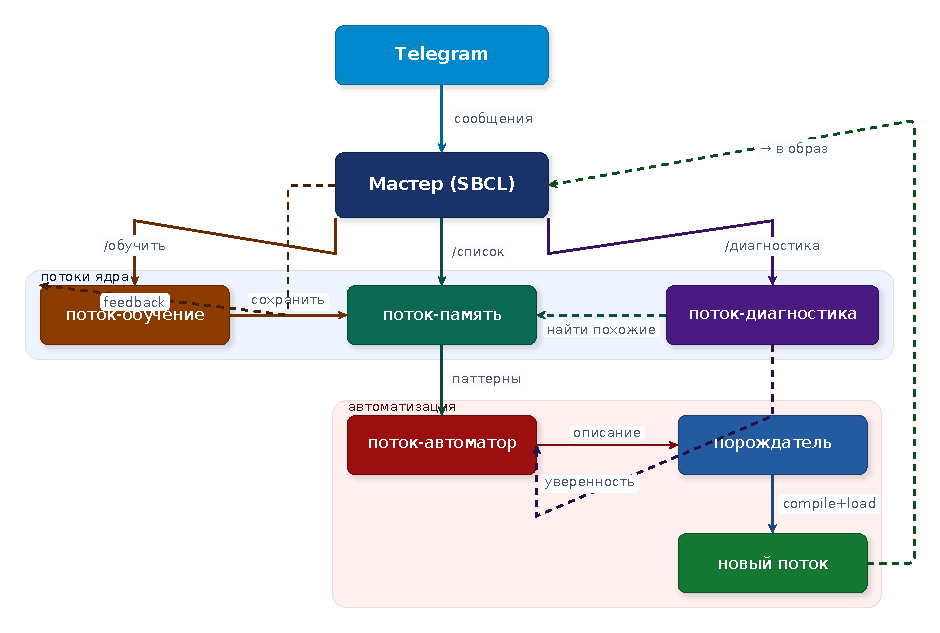
\includegraphics[width=\linewidth]{arch_diagram.pdf}
  \caption{Архитектура системы}
\end{figure}

\subsection{Поток \texttt{память}}

Долговременное хранилище (проблема $\to$ решение).

\textbf{Команды:}
\begin{lstlisting}[language={},numbers=none]
память добавить: проблема=... | решение=...
память найти: медленный queryset
память список
память удалить: 3
\end{lstlisting}

\textbf{Формат JSON:}
\begin{lstlisting}[language=JSON,caption={Структура памяти}]
{
  "id": 1,
  "проблема": "N+1 в GeoDjango",
  "решение": "select_related + prefetch",
  "теги": ["django", "n+1"],
  "оценка": 1,
  "применений": 3,
  "паттерн": "orm-n+1"
}
\end{lstlisting}

\textbf{Стратегии поиска:}

\begin{tabular}{@{}cll@{}}
  \toprule
  \# & Стратегия & Качество \\
  \midrule
  1 & Keyword matching & Низкое \\
  2 & LLM-сравнение & Среднее \\
  3 & Embedding + cosine & Высокое \\
  \bottomrule
\end{tabular}

\textit{MVP: стратегия~2.}

\subsection{Поток \texttt{обучение}}

Принимает пару, валидирует, сохраняет, анализирует паттерн.

\begin{lstlisting}[language={},numbers=none]
проблема: N+1 при обходе Route.objects.all()
решение: Route.objects.prefetch_related('waypoints')
теги: django, n+1
\end{lstlisting}

Логика: парсинг → проверка дубликатов → сохранение → анализ паттерна (новый / вариация).

\subsection{Поток \texttt{диагностика}}

При новой проблеме ищет похожие, предлагает решение с уверенностью.

\begin{tabular}{@{}cll@{}}
  \toprule
  \textbf{\%} & \textbf{Статус} & \textbf{Действие} \\
  \midrule
  85--100 & Высокая & Автоматизировать \\
  70--84  & Хорошая & Попробовать \\
  50--69  & Средняя & Проверить \\
  0--49   & Низкая  & Гипотеза \\
  \bottomrule
\end{tabular}

\subsection{Поток \texttt{автоматор}}

Мониторит паттерны, при достижении порогов предлагает породить специализированный поток.

\textbf{Триггеры:}
\begin{itemize}
  \item Уверенность $\geq 85\%$
  \item Паттерн встречался $\geq 3$ раз
  \item Подтверждений $\geq 2$
\end{itemize}

% ═══════════════════════════════════════════════════════════════════
\section{Пример end-to-end}

\subsection{GeoDjango: 10 дней}

\textbf{День 1 --- обучение:}
\begin{lstlisting}[language={},numbers=none]
> /обучить
проблема: N+1 при Region.objects.all()
          с доступом к region.city
решение: select_related('city')

< Сохранено (id=1). Новый паттерн.
\end{lstlisting}

\textbf{День 3:}
\begin{lstlisting}[language={},numbers=none]
> /обучить
проблема: Медленный Point + prefetch Polygon
решение: prefetch_related + .only('id','geom')

< Сохранено (id=2). Схоже с id=1.
  Паттерн: "ORM оптимизация"
\end{lstlisting}

\textbf{День 7 --- диагностика:}
\begin{lstlisting}[language={},numbers=none]
> /диагностика
  Route.objects.all() + route.waypoints.all()

< Найдено 2 похожих.
  РЕШЕНИЕ: prefetch_related('waypoints')
  УВЕРЕННОСТЬ: 87%
  Применить? [да/нет]

> да
< Паттерн "orm-n+1": 3 случая, 100%.
  Рассматриваю автоматизацию...
\end{lstlisting}

\textbf{День 10 --- автоматизация:}
\begin{lstlisting}[language={},numbers=none]
< Устойчивый паттерн: N+1 в Django ORM
  5 случаев, 100%, ср. уверенность 89%

  Создать поток «оптимизатор-orm»?

> да
< Поток загружен в образ.
\end{lstlisting}

\begin{successbox}[title={Итог}]
10 дней от нуля до специализированного
автоматического потока.
\end{successbox}

% ═══════════════════════════════════════════════════════════════════
\section{Реализация}

\subsection{Поток \texttt{память}}

\begin{lstlisting}[language=CommonLisp,caption={поток-память.lisp}]
(defpackage :поток-память
  (:use :cl)
  (:export #:выполнить #:добавить-пример
           #:найти-похожие #:получить-все
           #:удалить-пример #:обновить-оценку))

(in-package :поток-память)

;;; LLM-сравнение двух проблем
(defun похожи-p (п-1 п-2)
  (let* ((pr (format nil
               "А: ~A~%Б: ~A~%Похожи? да/частично/нет"
               п-1 п-2))
         (r (string-downcase (llm-запрос pr))))
    (cond ((search "да"       r) :да)
          ((search "частично" r) :частично)
          (t                     :нет))))

;;; Поиск k ближайших
(defun найти-похожие (проблема &key (k 3))
  (let* ((scored
          (mapcar (lambda (п)
            (cons (похожи-p проблема
                    (cdr (assoc :проблема п)))
                  п))
            (примеры)))
         (sorted
          (sort scored
            (lambda (a b)
              (> (case (car a)
                   (:да 2) (:частично 1) (t 0))
                 (case (car b)
                   (:да 2) (:частично 1) (t 0)))))))
    (remove-if (lambda (x) (eq (car x) :нет))
      (subseq sorted 0 (min k (length sorted))))))

(defun выполнить (задача)
  (handler-case
    (let ((cmd (парсить-команду задача)))
      (case (first cmd)
        (:добавить
          (format nil "Сохранено (id=~A)"
            (добавить-пример (second cmd)
                             (third cmd))))
        (:найти
          (форматировать-результаты
            (найти-похожие (second cmd))))
        (:список
          (форматировать-список (получить-все)))
        (:удалить
          (удалить-пример (second cmd)))))
    (error (e) (format nil "Ошибка: ~A" e))))
\end{lstlisting}

\subsection{Self-critique в диагностике}

\begin{lstlisting}[language=CommonLisp,caption={Двухэтапная диагностика}]
(defun диагностика-с-критикой (проблема)
  (let* ((похожие
          (поток-память:найти-похожие проблема :k 5))
         (решение
          (сгенерировать-решение проблема похожие))
         (критика
          (llm-запрос
           (format nil
             "Решение: ~A~%Проблема: ~A~%~
              1. Решает проблему?~%~
              2. Побочные эффекты?~%~
              3. Нужны уточнения?"
             решение проблема))))
    (format nil "~A~%~%Самопроверка:~%~A"
            решение критика)))

(defun извлечь-уверенность (ответ)
  (let ((p (search "УВЕРЕННОСТЬ:"
                   (string-upcase ответ))))
    (if p
        (parse-integer
         (remove-if-not #'digit-char-p
           (subseq ответ (+ p 12) (+ p 15))))
        50)))
\end{lstlisting}

\subsection{Автоматор: порог и порождение}

\begin{lstlisting}[language=CommonLisp,caption={поток-автоматор.lisp}]
(defparameter *мин-случаев*    3)
(defparameter *мин-успешность* 0.8)

(defun готов-p (stat)
  (and (>= (getf stat :случаев)    *мин-случаев*)
       (>= (getf stat :успешность) *мин-успешность*)
       (>= (getf stat :применений)
           (* 2 (getf stat :случаев)))))

(defun породить (stat)
  (поток-порождатель:выполнить
   (format nil
     "Создай поток ~A-оптимизатор.~%~
      Паттерны:~%~{- ~A -> ~A~%~}"
     (getf stat :название)
     (mapcan (lambda (п)
               (list (cdr (assoc :проблема п))
                     (cdr (assoc :решение п))))
             (subseq (getf stat :примеры) 0 5)))))
\end{lstlisting}

% ═══════════════════════════════════════════════════════════════════
\section{Эволюция и обратная связь}

\subsection{Lifecycle}

\begin{tabular}{@{}cll@{}}
  \toprule
  \textbf{Этап} & \textbf{N} & \textbf{Поведение} \\
  \midrule
  Накопление    & $<3$   & Только сохранение \\
  Имитация      & $3-10$ & Few-shot решения \\
  Обобщение     & $10+$  & Абстрактные паттерны \\
  Автоматизация & крит.  & Порождение потока \\
  \bottomrule
\end{tabular}

\subsection{Feedback}

\begin{lstlisting}[language={},numbers=none]
/хорошо 5        -- +1 к оценке id=5
/плохо 5 "не то" -- -1, сохранить антипаттерн
\end{lstlisting}

Антипаттерн сохраняется с префиксом «НЕ ДЕЛАТЬ:» и учитывается в диагностике.

\subsection{Защита от деградации}

\begin{enumerate}
  \item \textbf{Decay} --- влияние примеров без применений снижается через 30 дней
  \item \textbf{Порог применений} --- мин.~2 успешных до автоматизации
  \item \textbf{Self-critique} --- LLM оценивает паттерн перед порождением
  \item \textbf{Карантин} --- новые потоки первые 5 вызовов требуют подтверждения
\end{enumerate}

% ═══════════════════════════════════════════════════════════════════
\section{Roadmap}

\subsection{День 1 --- MVP}

\begin{lstlisting}[language=CommonLisp,caption={Поиск без LLM для быстрого старта}]
(defun найти-по-словам (проблема примеры)
  (let ((слова (uiop:split-string
                 (string-downcase проблема))))
    (sort примеры #'>
      :key (lambda (п)
        (count-if (lambda (с)
          (search с (string-downcase
            (cdr (assoc :проблема п)))))
          слова)))))
\end{lstlisting}

\begin{itemize}
  \item[\checkmark] поток-память с keyword matching
  \item[\checkmark] добавление, поиск, список
  \item[\checkmark] тест: 3 примера + поиск
\end{itemize}

\subsection{Неделя 1}
\begin{itemize}
  \item LLM-поиск по сходству
  \item поток-обучение, поток-диагностика
  \item feedback (/хорошо, /плохо)
\end{itemize}

\subsection{Неделя 2}
\begin{itemize}
  \item поток-автоматор
  \item интеграция с порождатель
  \item карантин, тест end-to-end
\end{itemize}

\subsection{Месяц 1}
\begin{itemize}
  \item self-critique, decay
  \item UI просмотра памяти
  \item статистика и метрики
\end{itemize}

\subsection{Долгосрочно}
\begin{itemize}
  \item Embedding-поиск (локальная модель)
  \item Иерархия паттернов
  \item LSP-расширение для IDE
\end{itemize}

% ═══════════════════════════════════════════════════════════════════
\section{Риски}

\begin{tabular}{@{}p{18mm}p{40mm}@{}}
  \toprule
  \textbf{Риск} & \textbf{Митигация} \\
  \midrule
  Контекстное окно
    & Топ-5 примеров, batch-сравнение \\[3pt]
  Drift качества
    & Decay, тегирование версий \\[3pt]
  Overfitting
    & Self-critique + флаг «проверено» \\[3pt]
  Безопасность кода
    & Sandbox, timeout, карантин \\[3pt]
  Стоимость LLM
    & Batch, кэш, дешёвая модель \\
  \bottomrule
\end{tabular}

\vspace{4pt}
\textbf{Стоимость поиска:}
$100 \times \approx5\text{ токенов} \approx \$0.001$ --- приемлемо.

% ═══════════════════════════════════════════════════════════════════
\section{Заключение}

\begin{enumerate}
  \item \textbf{ICL достаточен} --- fine-tuning избыточен и вреден
  \item \textbf{Метациркулярность} --- порождатель уже есть, это его расширение
  \item \textbf{Gradual autonomy} --- от имитации к автоматизации постепенно
  \item \textbf{Human-in-the-loop} --- без feedback система деградирует
\end{enumerate}

\begin{successbox}[title={Через месяц система успешна, если:}]
\begin{itemize}
  \item Меньше времени на повторяющиеся задачи
  \item Хотя бы 1 авто-порождённый полезный поток
  \item Точность предложений $> 70\%$
\end{itemize}
\end{successbox}

\subsection{Первые шаги}

\begin{enumerate}
  \item Скопировать скелеты (раздел~5) в \texttt{мастер/потоки/}
  \item Добавить 5 реальных примеров из практики
  \item Использовать, давать feedback, наблюдать
\end{enumerate}

\vfill
\vspace{4mm}
{\color{AccentBlue}\rule{\linewidth}{0.4pt}}
{\fontsize{6.5}{8}\color{MidGray}
  Версия~1.0 · 14~марта~2026 · \texttt{development\_system}
}

\end{document}
